\beginsong{Die Moorsoldaten}[mel={Rudi Goguel, Hans Eigler, 1933}, txt={Johann Esser, Wolfgang Langhoff, 1933}, bo={420}, pfii={68}, pfiii={42}, index={Wohin auch das Auge blicket}]

\markboth{\songtitle}{\songtitle}

\beginverse
\endverse

\centering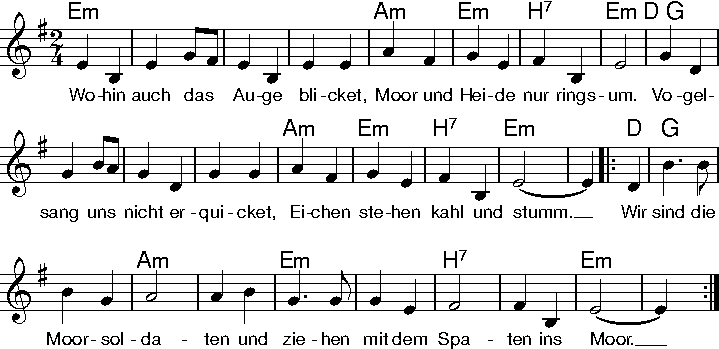
\includegraphics[width=1\textwidth]{Noten/Lied025.pdf}	

\beginverse
\[Em]Hier in dieser öden Heide \[Am]ist das \[Em]Lager \[H7]aufge\[Em]baut, \[D]
\[G]wo wir fern von jeder Freude \[Am]hinter \[Em]Stachel\[H7]draht ver\[Em]staut.
\endverse

\beginchorus
\lrep \[D]Wir \[G]sind die Moorsol\[Am]daten und \[Em]ziehen mit dem \[H7]Spaten ins \[Em]Moor! \rrep
\endchorus

\beginverse
^Morgens ziehen die Kolonnen ^in das ^Moor zur ^Arbeit ^hin, ^
^Graben bei dem Brand der Sonne, ^doch zur ^Heimat ^steht der ^Sinn.
\endverse
%\renewcommand{\everychorus}{\textnote{\bf Refrain (wdh.)}}
\beginchorus
\lrep \[D]Wir \[G]sind die Moorsol\[Am]daten und \[Em]ziehen mit dem \[H7]Spaten ins \[Em]Moor! \rrep
\endchorus
\beginverse
^Heimwärts, heimwärts! Jeder sehnet ^sich nach ^Eltern, ^Weib und ^Kind. ^
^Manche Brust ein Seufzer dehnet, ^weil wir ^hier ge^fangen ^sind.
\endverse

\beginchorus
\lrep \[D]Wir \[G]sind die Moorsol\[Am]daten und \[Em]ziehen mit dem \[H7]Spaten ins \[Em]Moor! \rrep
\endchorus

\beginverse
^Auf und nieder geh'n die Posten; ^keiner, ^keiner ^kann hin^durch. ^
^Flucht wird nur das Leben kosten, ^vierfach ^ist um^zäunt die ^Burg.
\endverse

\beginchorus
\lrep \[D]Wir \[G]sind die Moorsol\[Am]daten und \[Em]ziehen mit dem \[H7]Spaten ins \[Em]Moor! \rrep
\endchorus

\beginverse
^Doch für uns gibt es kein Klagen, ^ewig ^kann's nicht ^Winter ^sein. ^
^Einmal werden froh wir sagen: ''^Heimat, ^Du bist ^wieder ^mein!''
\endverse

%\renewcommand{\everychorus}{\textnote{\bf Refrain}}
\beginchorus
\lrep \[D]Dann \[G]zieh'n die Moorsol\[Am]daten \[Em]nicht mehr mit dem \[H7]Spaten in's \[Em]Moor! \rrep
\endchorus

\endsong

\beginscripture{}
Das Lied entstand 1933 im Konzentrationslager Börgermoor (im Emsland), in dem hauptsächlich politische Gefangene untergebracht waren. Obwohl die Lagerleitung es schnell verbot, beförderte das Wachpersonal den Gesang des Liedes. Es wurde auch in anderen Moorlagern gesungen und von entlassenen Häftlingen verbreitet, sodass es sogar der Moskauer Rundfunk zu Ehren deutscher Antifaschisten spielte.
\endscripture

\begin{intersong}
\end{intersong}